\documentclass{article}

\usepackage[final]{neurips_2019}
\usepackage[utf8]{inputenc} % allow utf-8 input
\usepackage[T1]{fontenc}    % use 8-bit T1 fonts
\usepackage{url}            % simple URL typesetting
\usepackage{booktabs}       % professional-quality tables
\usepackage{amsfonts}       % blackboard math symbols
\usepackage{nicefrac}       % compact symbols for 1/2, etc.
\usepackage{microtype}      % microtypography
\usepackage{graphicx}
\usepackage{subfig}
\usepackage{natbib}
\usepackage{float}
\usepackage{array}
\usepackage{algpseudocode, algorithm}
\usepackage{amsmath}
\usepackage{multicol}
\setlength{\columnsep}{1cm}

\usepackage{hyperref}
\hypersetup{
    colorlinks=true,
    linkcolor=blue,
    filecolor=magenta,      
    urlcolor=cyan,
}

\usepackage{caption}
\captionsetup[table]{labelsep=space}
\captionsetup[figure]{labelsep=space}
\newcommand{\mycaption}[2]{\caption[#1]{\textbf{#1.} #2}}

\title{Residual Attention Network for Image Classification}

\author{%
  Shengjie Sun \\
  ss5593\\
  Department of Statistics\\
  Columbia University\\
  \texttt{ss5593@columbia.edu} \\
  % examples of more authors
  \And
  Yiming Tan \\
  yt2658 \\
  Department of Statistics\\
  Columbia University\\
  \texttt{yt2658@columbia.edu} \\
  \And
  Feng Su \\
  fs3658 \\
  Department of Statistics\\
  Columbia University\\
  \texttt{fs3658@columbia.edu}
}

\begin{document}

\maketitle

\begin{multicols}{2}
\section*{Abstract}
\textit{In this project, we reimplement a convolutional neural network structure called "Residual Attention Network" proposed by \citet{wang2017residual}. The great power of attention in machine translation has indicated by \citet{vaswani2017attention} and thus we are curious about how the idea of attention can influence the image classification task. The main challenging of implementation is that the attention part of network is too flexible to choose a good hyper-parameters and the time and computing resources is limited for this project. Finally, our implementation on CIFAR dataset got $90\%$ percentage of accuracy of the paper but we still argued the idea of this paper maybe not a good choice for CIFAR-10 and CIFAR-100.}





\section{Introduction}
As \citet{wang2017residual} mentioned that the residual mechanism in the image classification can serve to both focused location selection and the enhancement of the representations of focused objects. After the network structure like VGG given by \cite{simonyan2014very} and the improvement of computing resources, the newer networks are mostly deeper. Basically, residual attention network is a very deep convolutional neural network connected by residual unit mixed with soft mask, so called attention in this paper. 

As for our project, we want to implement the idea of this paper in tensorflow 2 and then compared our result and the result in the paper. Furthermore, we try to exam what should be a good "attention" for the image classification, the attention mentioned in this paper is actually a soft mask, which is quite different from the word "attention" used in the area of natural language processing. 
\end{multicols}

\begin{figure}[!htb]  
\centering  
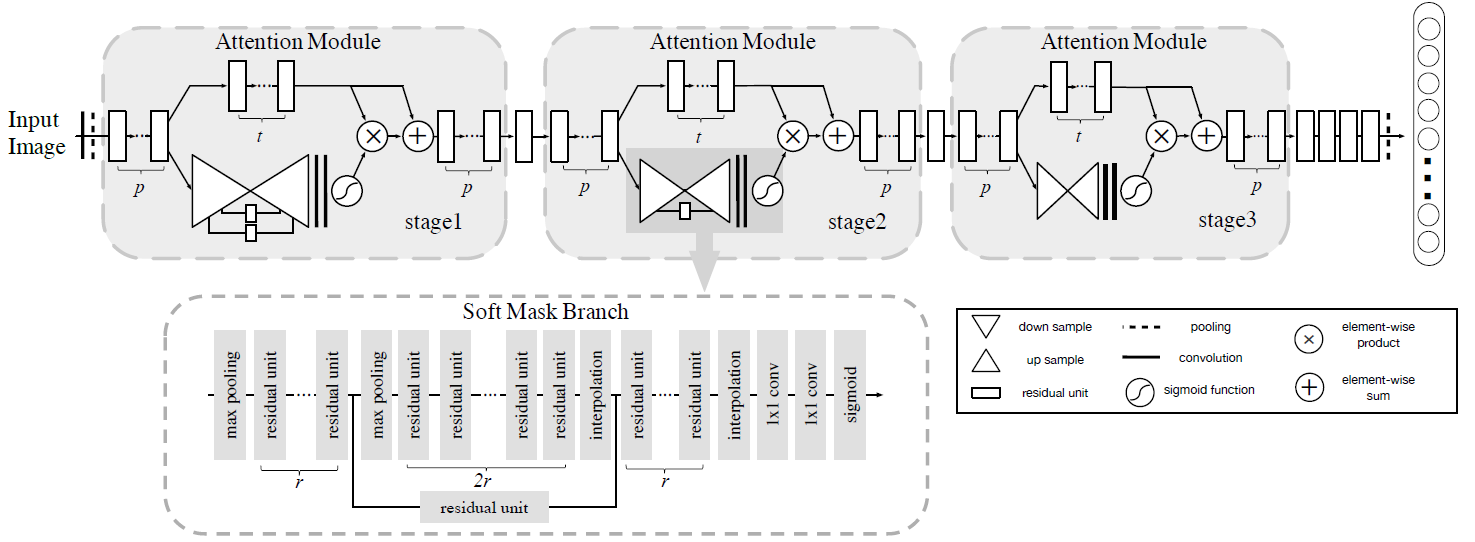
\includegraphics[width=6in]{imgs/attention_module_stage2.png}  
\mycaption{Example architecture of the residual attention network.}{We use three hyper-parameters for the design of Attention Module: p, t and r. The hyper-parameter p denotes the number of pre-processing Residual Units before splitting into trunk branch and mask branch. t denotes the number of Residual Units in trunk branch. r denotes the number of Residual Units between adjacent pooling layer in the mask branch. In our experiments, we use the following hyper-parameters setting: {p = 1, t = 2, r = 1}. The number of channels in the soft mask Residual Unit and corresponding trunk branches is the same.}  
\label{fig:attention_module_stage2}
\end{figure}

\newpage
\begin{multicols}{2}
There are several challenges and difficulties. First of all, so many implementation details are not provided by the original paper. The details of a residual unit is not clear. The second main challenging is the limited time. Training the model one time is not such time consuming but as we said, the structure of this kind of network is flexible and thus we have so many hyper-parameters to tune. The third one is over-fitting, during training, we found the model tended to over fit the dataset.

Our solution to the first difficulty is to give a model with similar size of parameters. Even thought there are many details, the skeleton of the structure is clear. Therefore, we tried to give an implementation with similar size of parameters. The solution to the second one is that we tried as many acceleration methods as we can to squeeze our computation ability. And we also sacrificed some accuracy based on the real situation. We tried all the method learnt from class but there is still a little bit overfitting. 





\section{Summary of the Original Paper}

\subsection{Methodology of the Original Paper}
The key idea of the whole paper lies on the structure of attention module and it can be roughly summarized by the following formula:
\begin{eqnarray*}
H_{i,c}(x)&=&(1+M_{i,c}(x))*T_{i, c}(x) \\
&=&T_{i, c}(x) + M_{i,c}(x)*T_{i, c}(x)
\label{eqn:attention_module}
\end{eqnarray*}
$T(x)$ is the common feed forward layers while the elements in $M(x)$ ranges from [0, 1] and serves as feature selectors. 

If we consider $M_{i,c}(x)*T_{i, c}(x)$ as $x$, it would be exactly the same as residual learning. But it is indeed based on attention structure, and thus called residual attention network.

\begin{figure}[H] 
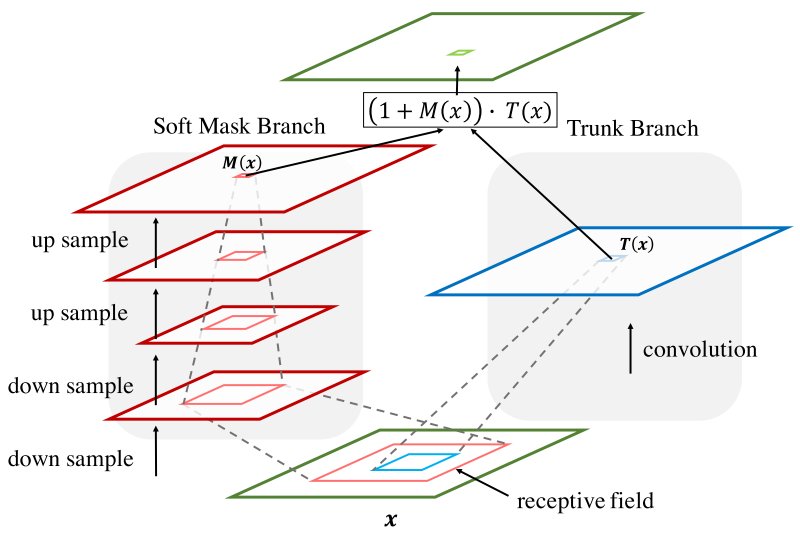
\includegraphics[width=3in]{imgs/receptive_field.png}  
\mycaption{Structure of Attention Module.}{$T(x)$ indicates the features generated by deep convolutional networks. $M(x)$ is the mask branche which work as feature selectors that enhance good features and suppress noises from trunk features.}  
\label{fig:receptive_field}
\end{figure}

\subsection{Key Results of the Original Paper}

\subsubsection{Residual structure benefits}
This paper argues that utilizing residual structure enables the stacking of more attention modules as shown in Figure \ref{fig:cifar10_residual}. This is not surprising too much as this is just why residual learning, i.e. skipping connection, is so popular and useful.
\begin{figure}[H] 
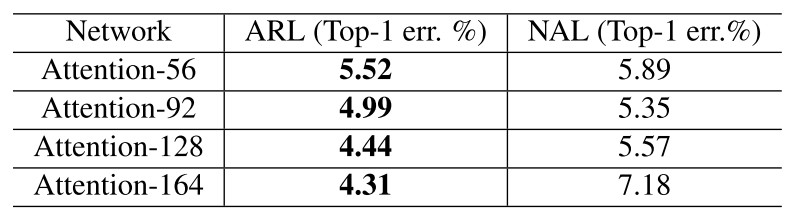
\includegraphics[width=3in]{imgs/cifar10_residual.png}  
\mycaption{Classification error (\%) on CIAFR-10.}{The networks trained using attention residual learning technique consistently outperform the networks trained with baseline method. The performance increases with the number of attention module when applying attention residual learning. In contrast, the performance of networks trained with “naive attention learning” method suffers obvious degradation.}  
\label{fig:cifar10_residual}
\end{figure}
The Figure \ref{fig:cifar10_stages} proved above argument in details, we can see that residual attention model has similar relative mean response to ResNet-164.
\begin{figure}[H] 
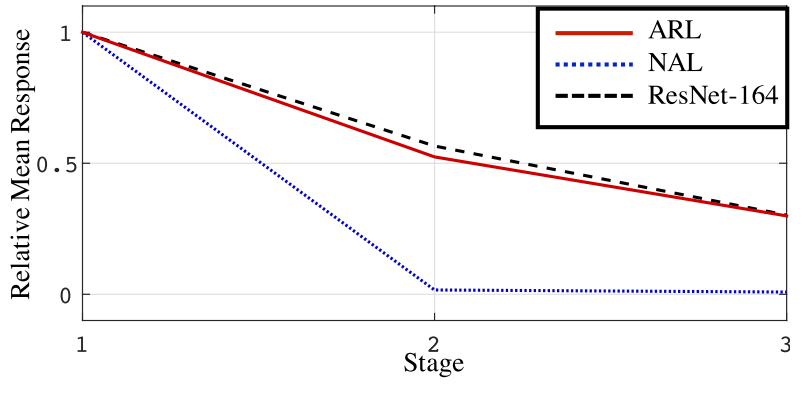
\includegraphics[width=3in]{imgs/cifar10_stages.png}  
\mycaption{The mean absolute response of output features in each stage.}{The response generated by the network trained using naive attention learning quickly vanishes in the stage 2 after four attention modules compared with network trained using attention residual learning.}  
\label{fig:cifar10_stages}
\end{figure}

\subsubsection{Attention structure benefits}
The paper shows that their model outperforms the state of art models. On the dataset CIFAR-10 and CIFAR-100, the attention residual learning scheme can effectively reduce the number of parameters in the network while enhancing the accuracy of the classification.
\begin{figure}[H] 
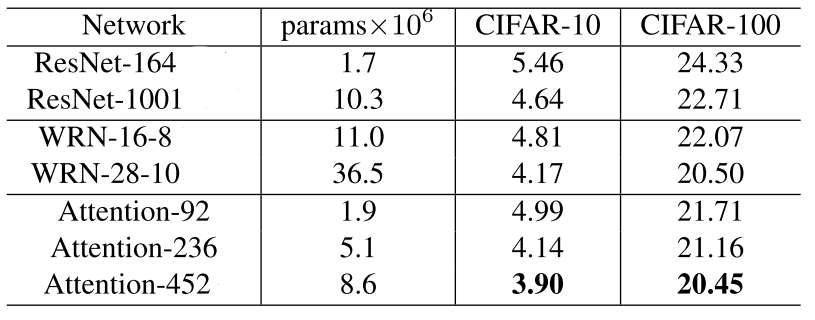
\includegraphics[width=3in]{imgs/cifar10_modes}  
\mycaption{Comparisons with state-of-the-art methods on CIFAR-10/100}{}
\label{fig:cifar10_modes}
\end{figure}





\section{Methodology}
Basically, the model is constructed by attention modules shown in Figure \ref{fig:attention_module_stage2}. One attention module has two branches: trunk branch and soft mask branch. At each stage, there could be several attention modules and in Figure \ref{fig:attention_module_stage2}, each stage contains exactly one module. More specifically, in the soft mask branch, there are different number of skip connections between down sampling and up sampling layers. 
 
\subsection{Objectives and Technical Challenges}
The paper did not provide the details of the residual unit and up or down sampling layers. But for the reimplementation, these details are crucial. In our project, we tried to build Attention56 for CIFAR-10, i.e. in each stage, there is only one attention module. The soft mask branch has two skip connections at stage 1, one skip connection at stage 2 and one at the last stage which is exactly same to to the Figure \ref{fig:attention_module_stage2}. 

The main object is to get the accuracy as close as the one provided in the paper. But as mentioned several times, the details is important but hidden in this paper, so lots of experiments required but the time and computing resources limited. 

The other challenge is the coding writing, it is not difficult to build the overall structure for a specific model, say Attention56. But it is super time consuming to adjust the hyper-parameters. It is quite clear there are lots of sampling steps and skip connections. Therefore the dimension and the shape of images/tensors become a little bit annoying to keep consistent. Besides, the different model requires different attention model, at the end, the dimensions become chaos and requires lot of time to adjust. So, if you want to give codes which can reused for many models, it is somehow difficult to design. If not, there will be plenty of repeating codes that fixed the inputs and outputs dimension for each layers. 

The last but not least is how to prevent over-fitting. The learning ability of these model are high and over-fitting is common. Even there are so many skip connections, the over-fitting is still obvious. Finding a good way to prevent it for this kind of model structure is difficult for us. 

\subsection{Problem Formulation and Design}
The main  goal is to reimplement the idea of residual attention net proposed by the paper. The whole residual attention neural network mainly consists of three attention modules, so the main challenge in implementation is to construct all the components in the attention module. The overall software design is shown in Figure \ref{fig:architect}, where three attention module objects are used in the residual attention network. 

Within the Attention Module class, a MaskBranch class and a TrunkBranch class is built to implement each branch. To build up these two branch classes, several basic units are used. DownSampleUnit, UpSampleUnit and ReidualUnitIdentity are three classes used to construct the MaskBranch, while the TrunkBranch class is a block of ResidualUnit objects. 
\begin{figure}[H] 
\includegraphics[width=3in]{imgs/Architect.png}  
\mycaption{The architecture of the whole model}{}  
\label{fig:architect}
\end{figure}
The further details about the implementation in shown in the next section. 

In order to check whether the residual structure can enhance the number of stacking attention module, we exam the weights and gradient during the training process which is discussed in the result section. 





\section{Implementation}

\subsection{Deep Learning Network}
The architectural diagrams are Figure \ref{fig:architect} and Figure \ref{fig:attention_module_stage2}. 
As for the training details, it is shown in Figure \ref{fig:training flowchart} in Appendix. The general parameters are \textbf{epoch and batch}: a maximum of 300 epochs with a batch size of 128 in each epoch is used in training. If the early stopping condition is not satisfied, the model would be trained in at most 300 epochs. \textbf{Learning rate and decay}: a decaying learning rate with patience is used. The learning rate is .001, if the validation accuracy can not be improved in 10 epochs, a factor of .6 will be multiplied to the learning rate. \textbf{Data Augmentation}: for data augmentation, horizontal and vertical flipping on the original pictures is done.
\textbf{Early stopping}: early stopping is introduced here by checking the validation accuracy of the model. If the best validation accuracy could not be improved in 20 epochs, the training would be stopped.



In the following part, we will give details of how the mask and truck brunches are implemented. 

\textbf{Mask Branch Implementation}. The algorithm design of Mask Branch is shown in Figure \ref{fig:mask_flowchart}. The input of this branch first goes through a loop of down-sampling units until all the down-sampling units are done. After each down-sampling unit, the output is put into an identity list for later use in skip connections. After all the up-sampling units are done, a similar loop consisting of corresponding up-sampling units is done until all the up-sampling units are finished. Before each up-sampling unit, the corresponding identity value in the identity list is added to the output to establish the skip connections between sampling layers. After all the up-sampling units are completed, the output information then go through two convolutional layers and a sigmoid activation function before it is returned as the output of this branch.
\begin{figure}[H] 
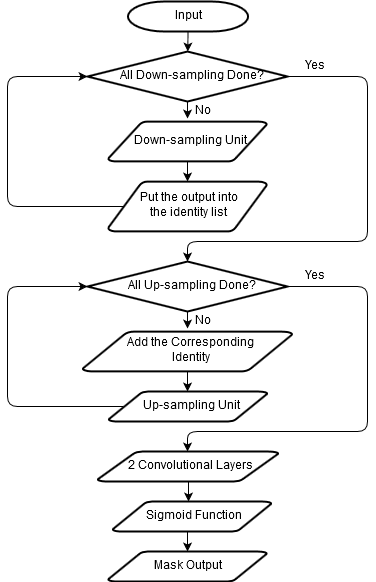
\includegraphics[width=3in]{imgs/mask_flowchart.png}  
\mycaption{Mask Branch in an Attention Module}{}  
\label{fig:mask_flowchart}
\end{figure}

\textbf{Trunk Branch Implementation}. As shown in \ref{fig:trunk_flowchart}, the structure of Trunk Branch is easier and more straightforward. The input of the Trunk Branch goes through residual units until all the residual units defined in this branch all completed. The result after these residual units is then returned as the output of the Trunk Branch.
\begin{figure}[H] 
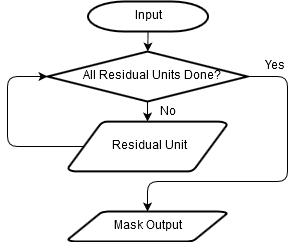
\includegraphics[width=3in]{imgs/trunk_flowchart.png}  
\mycaption{Trunk Branch in an Attention Module}{}  
\label{fig:trunk_flowchart}
\end{figure}

\subsection{Software Design}
The flow charts have been shown in Figure \ref{fig:architect}, Figure \ref{fig:trunk_flowchart} and Figure \ref{fig:mask_flowchart}. The details are shown clearly in the github repository, all the code are well commented. 

The following is an example of pseudo code of define a tensorflow class of a model.

\begin{figure}[H]
\centering
\begin{minipage}{3in}
\begin{algorithm}[H]
\caption{Class of the Residual Attention Model}
	\begin{algorithmic}[1]
	\Function{$\_\_init\_\_$}{$config$}
		\State $conv_0$ = layers.Conv2D
		\State $residualunit_0$ = layers.ResidualUnitBetween
		\State $stage_1$ = AttentionModule
		\State $residualunit_1$ = layers.ResidualUnitBetween
		\State $stage_2$ = AttentionModule
		\State $residualunit_2$ = layers.ResidualUnitBetween
		\State $stage_3$ = AttentionModule
		\State $residualunit_3$ = layers.ResidualUnitBetween
		\State $bn$ = layers.BatchNormalization
		\State $flatten$ = layers.Flatten
		\State $fc_1$ = layers.Dense
		\State $fc_2$ = layers.Dense
	\EndFunction
	
	\Function{$call$}{$inputs, training$}
        \State out = $residualunit_0$($conv0$(inputs))
        
        \State out = $residualunit_1$($stage_1$(out))
        \State out = $residualunit_2$($stage_2$(out))
        \State out = $residualunit_3$($stage_3$(out))

        \State out = $avepooling$($bn$(out))

        \State flatten = $flatten$(out)
        \State logits = $out$($fc_2$($fc_1$(flatten)))
        
        \State return logits
	\EndFunction
\end{algorithmic}
    \end{algorithm}
  \end{minipage}
\end{figure}





\section{Results}
\subsection{Project Results}
For this project, we mainly reimplemented the Attention56 on both CIFAR-10 and CIFAR-100. As shown in Figure \ref{fig:accuracy}, this is the training and validation accuracy of Attention56 on CIFAR-10. The best validation accuracy is 0.78. 
\begin{figure}[H] 
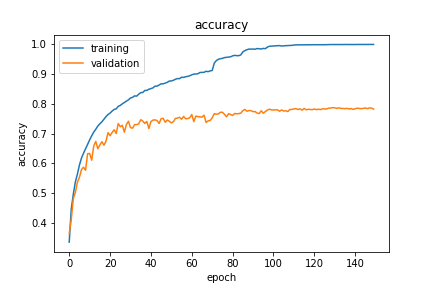
\includegraphics[width=3in]{imgs/accuracy.png}  
\mycaption{An Example of training and Validation history of Accuracy}{}  
\label{fig:accuracy}
\end{figure}

During the hyper-parameters tuning, the best validation accuracy on CIFAR-10 in 0.85 and 0.63 on CIFAR-100.

We also exam the weights of the last convolution kernel of mask branch at each stage as in Figure \ref{fig:hist}. We thought that the gradient back propagate well until before the first stage.
\begin{figure}[H]
  \centering
  \subfloat[Stage 1]{
  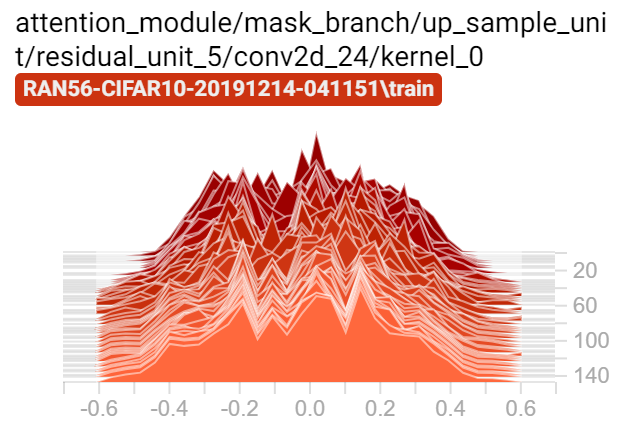
\includegraphics[width=1.4in]{imgs/attention_module_0.png}}
  \subfloat[Stage 2]{
  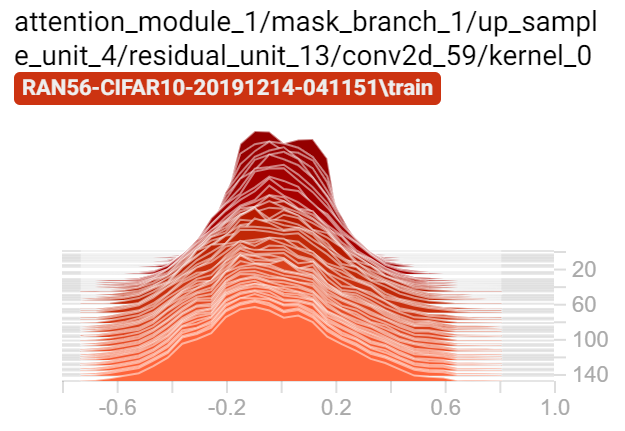
\includegraphics[width=1.4in]{imgs/attention_module_1.png}} \\
  \subfloat[Stage 3]{
  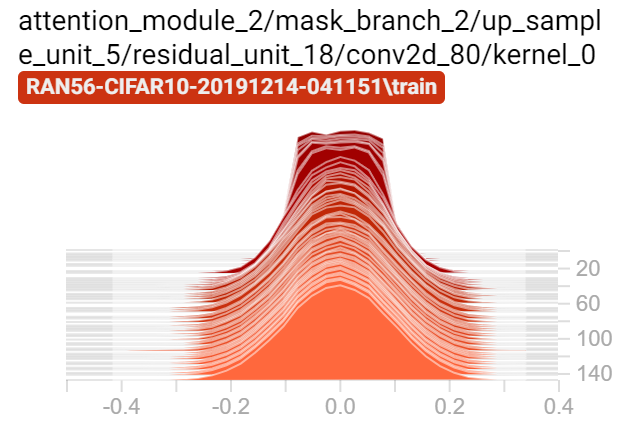
\includegraphics[width=2in]{imgs/attention_module_2.png}}
  \mycaption{The weights in the last layers of the three attention module}{}
  \label{fig:hist}
\end{figure}

\subsection{Comparison of Results}
As we can not get the ImageNet dateset, we can only compare the result on the 
CIFAR-10 and CIFAR-100. 
\begin{tabular}{ |p{1.4cm}||p{1.4cm}|p{1.4cm}|p{1.4cm}|  }
 \hline
 \multicolumn{4}{|c|}{Comparison of Results} \\
 \hline
 Models & params $\times 10^{6}$  & CIFAR-10 & CIFAR-100 \\
 \hline
 Our & $\leq1.9$ & 0.85 & 0.63 \\
 Paper & 2.7 & 0.94 & - \\
 \hline
\end{tabular}

The most critical problem for us is over-fitting shown in the follow Figure \ref{fig:loss}. It's may not clear in the Figure \ref{fig:accuracy} of accuracy but is obviously indicated by the loss. All the methods we learnt from class like regularization, reducing the capacity, dropout and so on has been tried, but can still reduce this kind of over-fitting.  
 
\begin{figure}[H] 
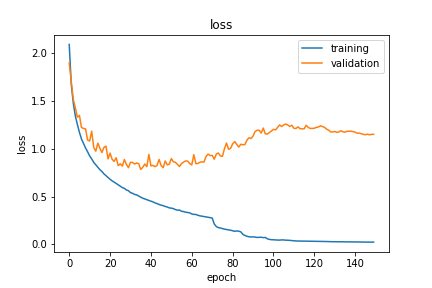
\includegraphics[width=3in]{imgs/loss.png}  
\mycaption{An Example of training and Validation history of Loss}{The yellow line is for validation loss, the over-fitting is clearly shown.}  
\label{fig:loss}
\end{figure}

\subsection{Discussion of Insights Gained}
Personally, this kind of structure is too flexible and required an elaborated setting of parameters, even the idea is quite easy to understand. The two dataset of the paper used is CIFAR-10\&100 and ImageNet. The project is done on CIFAR. The whole structure of network is following the paper, i.e the hyper-parameters related to the structure is set to be exactly same but other parameters and kernel size, stride size, epochs, etc. are not shown in the paper so we set by ourselves. 

The main problem is our model over-fitting a little bit. And thus our model's accuracy is about 0.1 lower than the original paper. 





\section{Conclusion}
We exam the idea of the residual attention which is a simple combination of attention and skip connection. At least for our project, \textbf{we don't think this is a good idea for the CIFAR dataset}, because first the dataset is small and most of the time, one picture for one object which means there is not so many things can distract the neural network. Therefore, attention maybe useless and the increase of number of parameters can even cause over-fitting. 

\textbf{We also don't think this is a good interpretation of the idea of attention in image classification.} The attention means soft mask in this paper which is quite different from that in the machine translation. First, no one argues that machine understand the picture in the same way as people and we do not know thoroughly what is the features extracted in the higher layer. Softmax is such rude way to intervene the features generated by the previous layers.

In the future, we tried to release the over-fitting further and exam the different interpretation of "attention" on image classification. 





\section{Appendix}
\subsection{Github Repository}
\href{https://github.com/cu-zk-courses-org/e4040-2019Fall-Project-SJST-ss5593-fs2658-yt2633}{https://github.com/cu-zk-courses-org/e4040-2019Fall-Project-SJST-ss5593-fs2658-yt2633}

\subsection{Individual Student Contributions}
\subsubsection*{Shengjie Sun (ss5593)}
{Fraction:} 
$5/12$
{What I did:} \\
Code the \texttt{residual.py}, \texttt{attention\_module.py}, \texttt{models.py}, \texttt{residual\_attention.ipynb}. \\
Report writing, model training and hyper-parameter tuning.

\subsubsection*{Yiming Tan (yt2658)}
{Fraction:} 
$4/12$
{What I did:} \\
Code the \texttt{attention\_module.py} and \texttt{models.py}. \\
Report writing, model training and hyper-parameter tuning.

\subsubsection*{Feng Su (fs3658)}
{Fraction:} 
$3/12$
{What I did:} \\
Report writing.

\subsection{Additional Diagrams}
\begin{figure}[H] 
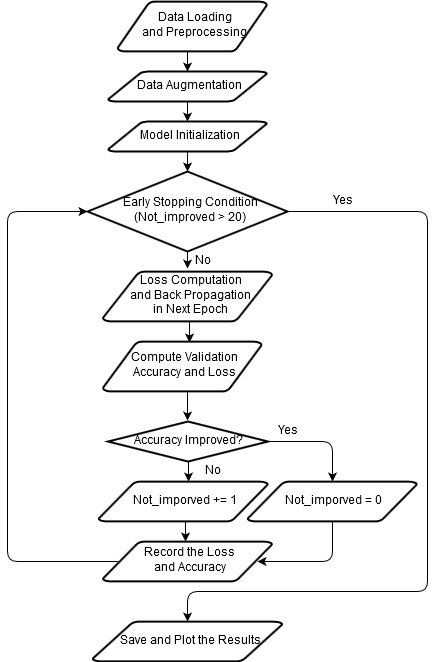
\includegraphics[width=3in]{imgs/training_flowchart.png}  \mycaption{Training Details}{}  
\label{fig:training flowchart}\end{figure}
\end{multicols}


\newpage

\bibliography{citations}
\bibliographystyle{plainnat}
\end{document}